\section{Sensitivity of passive BIC preparation and Floquet robustness}
\label{sec:k_sensitivity}

The preparation schemes based on a static Bell-BIC rely on a precise
phase-matching condition at the resonant wave vector \(K_0=\pi/2\). This
point is important because the Bell state is dark only when the collective
radiative amplitudes interfere destructively at the resonant mode. A small
shift \(K=K_0+\delta K\) therefore changes both the phase accumulated between
the coupling points and the collective decay matrix. To quantify this
limitation, we reproduce the passive Markovian benchmark used in the PRA
calculation, where the initial state
\begin{equation}
|\psi_K(0)\rangle =
\frac{|e,g\rangle-e^{-iK\Delta x}|g,e\rangle}{\sqrt{2}}
\end{equation}
is evolved under the collective Liouvillian defined by
\begin{equation}
A_{ij}(K)=
\frac{g^2}{2\xi}
\left[
2e^{iK|x_i-x_j|}
+e^{iK|x_i+n-x_j|}
+e^{iK|x_i-x_j-n|}
\right].
\label{eq:pra_collective_matrix}
\end{equation}
For \(K=K_0\) and \(\Delta x=2\), this state coincides with
\(|\Psi^+\rangle\). Away from \(K_0\), however, the target Bell state is no
longer protected by an exact dark condition and the fidelity decays under the
waveguide-induced collective dynamics.

Using the same parameters as the PRA diagnostic
\((g/\xi=0.5,n=8,\Delta x=2)\), the final fidelity at \(\xi t=500\)
already decreases to \(0.940\) for \(\delta K/K_0=0.005\) and to
\(0.782\) for \(\delta K/K_0=0.01\). For larger but still controlled
mismatches, the decay is essentially complete: \(F_{\Psi^+}=3.8\times10^{-3}\)
for \(\delta K/K_0=0.05\) and \(F_{\Psi^+}=1.1\times10^{-7}\) for
\(\delta K/K_0=0.10\). This behavior identifies the exact resonant
wave-vector condition as a practical bottleneck for passive Bell-state
storage.

Our Floquet protocol addresses this sensitivity in a different way. Rather
than relying on a Bell state that is passively protected after it has been
prepared, the drive actively follows a controlled dark-state path,
\begin{equation}
|D_a(\tau)\rangle =
\cos\theta(\tau)|e,g\rangle+\sin\theta(\tau)|g,e\rangle ,
\end{equation}
while the counterdiabatic term cancels the leading finite-time rotation
error. We test the same type of wave-vector mismatch by setting
\(\Omega(K)=\omega_c-2\xi\cos K\) and simulating the full finite-mode
central-sideband dynamics in the corresponding resonant rotating frame. The
figure below compares the passive benchmark with the two-stage Floquet
protocol.

\begin{figure*}[t]
\centering
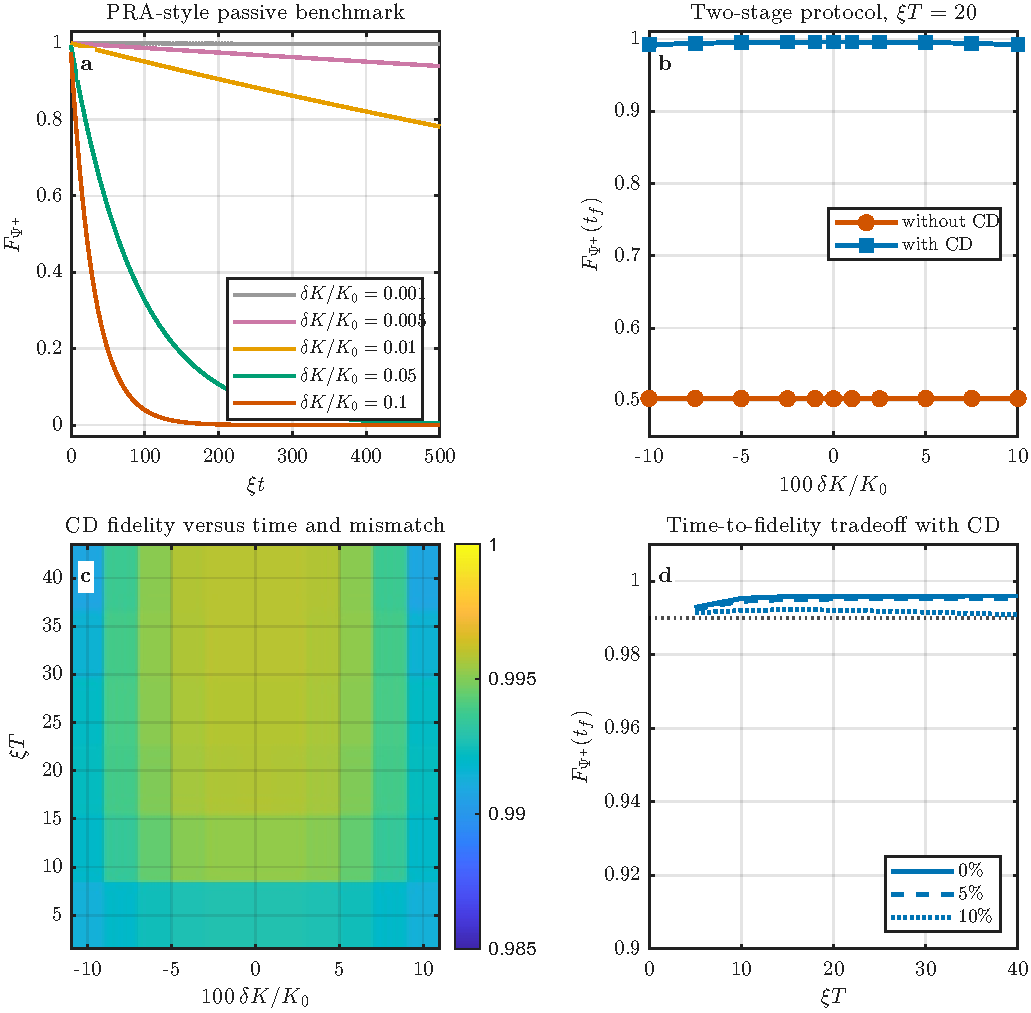
\includegraphics[width=\textwidth]{figures/Figure_K_Robustness_Comparison.pdf}
\caption{\textbf{Wave-vector sensitivity and robustness of the Floquet--CD
protocol.} \textbf{a,} Passive PRA-style benchmark: the fidelity with
\(|\Psi^+\rangle\) decays when the resonant wave vector is shifted away from
\(K_0=\pi/2\). \textbf{b,} Final Bell fidelity of the two-stage protocol at
\(\xi T=20\), with and without the counterdiabatic term. \textbf{c,} Final
Bell fidelity of the CD-assisted protocol as a function of passage time and
fractional wave-vector mismatch. \textbf{d,} Time-to-fidelity tradeoff for
selected mismatches.}
\label{fig:k_robustness_comparison}
\end{figure*}

The comparison shows that the static passive mechanism is highly sensitive to
the exact value of \(K\), whereas the driven protocol remains a high-fidelity
preparation method over the tested mismatch window. In the central-sideband
finite-mode calculation, the CD-assisted protocol at \(\xi T=20\) keeps
\(F_{\Psi^+}\ge 0.992\), \(\mathcal C\ge0.992\), and atomic population
\(P_{\rm at}\ge0.992\) throughout \(|\delta K|/K_0\le0.10\). The relevant
physical difference is that the Floquet--CD sequence does not wait for
dissipation to select the desired Bell component. Instead, a local
\(\pi\)-pulse first loads \(|e,g\rangle\), and the controlled couplings rotate
this excitation into the Bell component over a finite time. This gives an
explicit fidelity--time tradeoff and allows the operating point to be
optimized, rather than being fixed solely by the static phase-matching
condition.

We stress that this comparison is used as a sensitivity benchmark. The passive
calculation follows the Markovian PRA model, whereas the Floquet data are
obtained from the effective central-sideband Hamiltonian with counterdiabatic
control. A full laboratory-frame robustness analysis, including drive
imperfections and sideband leakage, will be required before claiming complete
microscopic robustness.
